\paragraph {}
Finalmente, con toda esta información, procedemos a desarrollar un protocolo de compensación de la ganancia. Nuestro objetivo es que, ante una modificación de la ganancia debido a una variación involuntaria de la temperatura (por ejemplo debido a variación climatológicas) aplicar de manera voluntaria una variación adecuada en el voltaje operacional que devuelva a la ganancia a su valor inicial.

\paragraph {}
Como ya se ha explicado la importancia de este estudio de compensación es poder utilizar este sistema a modo de alarma. Dado que este estará expuesto a condiciones climáticas inevitablemente sufrira variaciones de temperatura. Si queremos el detector final sea capaz de avisar en caso de obtener una señal demasiado grande y que esta señal se corresponda a una fuga de tritio necesitamos que el sistema posea una ganancia constante.

Las expresiones que se han obtenido con las dos calibraciones anteriores son:
$$G(V_{op})=cV_{op}+d; \qquad G(T)=aT+b$$

Esto implica que una variación de la ganancia en cada una de estas magnitudes viene reflejado como:
$$\partial G(V_{op}) = c \partial V_{op}; \qquad \partial G(T) = a \partial T$$

Finalmente, la variación total de la ganancia ante una variación de ambas magnitudes viene dado por:
$$\partial G_{tot} = \partial G(V_{op}) + \partial G(T)$$

Por tanto, si queremos que el valor de la ganancia se conserve ante una variación de ambas magnitudes tendremos que conseguir que: 
$$\partial G_{tot} = 0 =  \partial G(V_{op}) + \partial G(T) \longrightarrow \partial G(V_{op}) = -\partial G(T)  $$

En otras palabras, lo que tenemos que conseguir es producir la misma variación a la ganancia con la modificación del voltaje que la que se ha producido al variar la temperatura. Para determinar esta variarión únicamente sustituimos las expresiones anteriormente obtenidas para cada diferencial de la ganancia:
$$\partial G(V_{op}) = - \partial G(T)  \longrightarrow c \partial V_{op}= - a \partial T \longrightarrow  \partial V_{op}= - \frac{a}{c} \partial T$$

Finalmente consideramos que a y c las consideramos constantes en voltaje y temperatura, ya que, estas varian muy poco por lo que, en primera aproximación, es aceptable. Con ello integramos a cada lado y obtenemos:
$$\int_{V_i}^{V_f} \partial V_{op}= - \frac{a}{c} \int_{T_i}^{T_f}\partial T = - \frac{a}{c} \Delta T \longrightarrow \Delta V_{op}= e \Delta T$$

Donde se ha introducido un nuevo parámetro: $e=-\frac{a}{c}$ cuyo valor es:
$$c=2.34123 \cdot 10^8 \pm 2.55246 \cdot 10^6 \quad V^{-1}$$
$$a=-1.40308 \cdot 10^7 \pm 2.71545 \cdot 10^5 \quad T^{-1}$$
$$e=-\frac{a}{c} = 0.059929 \pm 0,001331$$
Donde el error de e se ha obtenido por propagación de errores. 
\paragraph {}
Finalmente, procedemos a analizar el resultado. Hemos obtenido dos dependencias de la ganancia lineales y opuestas. Por un lado la ganancia disminuye con la temperatura y por otro lado la ganancia aumenta con el voltaje operacional. Por tanto, si queremos conseguir modificaciones opuestas de la ganancia debemos desplazar voltaje y temperatura en la misma dirección (aumentar o disminuir ambas magnitudes simultaneamente). Si analizamos el resultado vemos que, efectivamente tenemos una dependencia positiva.

\paragraph {}
También apreciamos que obtenemos un valor dos ordenes de magnitud inferior a la unidad. Esto es debido a que la dependencia de la ganancia con el voltaje es mucho más marcada que la variación con la temperatura (mayor pendiente en valor absoluto para el ajuste del voltaje que para el ajuste de la temperatura). Este es el motivo por el que se tomo pasos inferiores para el voltaje que para la temperatura. 

\paragraph {}
En resumen la ecuación que nos dicta cual es la variación que debemos aplicar al voltaje para mantener un valor de ganancia constante (compensar la ganancia) ante una variación de la temperatura conocida (que puede ser medida con un sensor de temperatura) es:
$$\Delta V_{op}=0.059929 \cdot \Delta T$$

\paragraph {}
Finalmente tomamos como referencia el caso anteriormente mostrado en la sección de análisis de datos correspondiente a temperatura 25 grados, Humedad del 45\% y voltaje operacional de 53.97 V = $V_{BD}+ 3$ V, cuya ganancia habíamos visto que era $7.18235 \cdot 10^8$ y procedemos a realizar una verificación midiendo los casos de 21, 23, 25, 27 y 29 grados. En cada uno de ellos se corregirá el voltaje de alimentación de forma adecuada para mantener el mismo valor de la ganancia. El valor de la ganancia para cada caso se ve reflejado en la imagen veintiuno. 

\begin{figure}[hbtp]
\centering
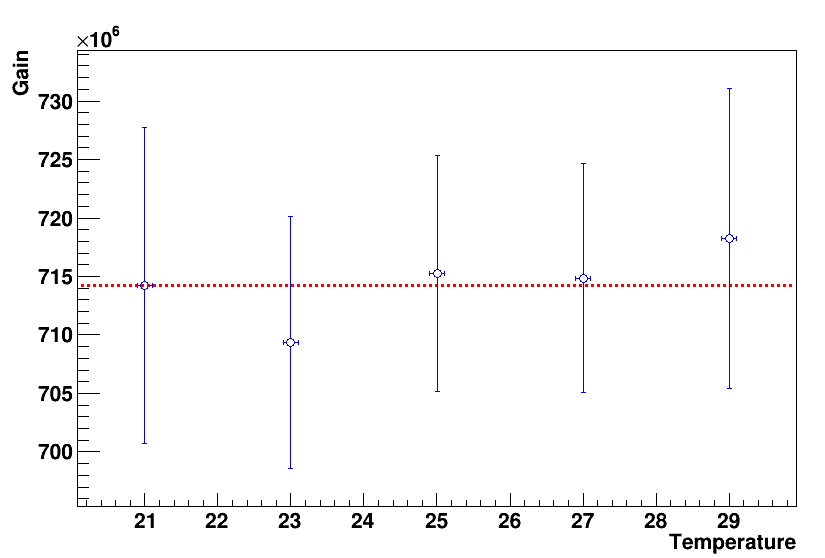
\includegraphics[scale=0.2]{/home/marcos/Documentos/Trabajo_final_de_Master/Trabajo/Figuras/compensacion.png}
\caption{\textbf{Imagen 21}.- Verificación del método de compensación}
\end{figure}

Donde la raya roja corresponde al ajuste a una constante. Su valor, correspondiente al valor de la ganancia es $G=7.14203 \cdot 10^8 \pm 4.97472 \cdot 10^6$

\paragraph {}
Podemos ver que el método funciona de manera muy eficaz ya que la ganancia presenta variaciones muy pequeñas de aproximadamente $\Delta G=5 \cdot 10^6$, que corresponde a una variación relativa del $2.801 \cdot 10^{-3} $. Vemos que es un método realmente eficaz.
\paragraph {}
La máxima variación se observo a 23 grados. Esta es debido a que fue una medida realizada muchas horas despues de tomarse las otras y existen factores externos que no podemos controlar y afectan al sistema. En este tiempo más largo transcurrido es más probable que hayan cambiado estos factores. Sin embargo puede observarse en todo momento que la variación de la ganancia es mínima verificando en gran medida la ecuación anteriormente obtenida.

\newpage